\chapter{Basi di Dinamica Topologica}

Consideriamo $T:X\to X$ con $X$ compatto e $T$ continua. Con la notazione $T^n$ intendiamo sempre la $n$-iterata di $T$.\\
Per semplicit\`a poniamo $\N^+=\N\nz$.

\section{Punti periodici e coniugio topologico}
\begin{definition}[Orbita]
Sia $x\in X$, l'\textbf{orbita} di $x$ \`e l'insieme
\[\Oc(x)=\cpa{T^n(x)}_{n\in\N}.\]
\end{definition}
\begin{definition}[Punto periodico]
Un punto $x\in X$ \`e \textbf{periodico} se esiste $m\in\N^+$ tale che $T^m(x)=x$.\\ 
Se $x$ \`e periodico chiamiamo \textbf{periodo minimo} il numero
\[p=\min\cpa{m\in \N^+ \mid T^m(x)=x}.\]
\end{definition}
\begin{remark}
Un \textbf{punto fisso} \`e un punto periodico di periodo minimo 1 (cio\`e $T(x)=x$).
\end{remark}
\begin{remark}
Se $x$ \`e periodico con periodo minimo $p$ allora $\Oc(x)=\cpa{x,T(x),\cdots,T^{p-1}(x)}$.
\end{remark}

\begin{definition}[Punti definitivamente periodici]
Un punto $x\in X$ si dice \textbf{definitivamente periodico} se esiste $m\in\N^+$, tale che $T^{m}(x)$ \`e periodico ma $x$ non lo \`e.
\end{definition}

\begin{remark}
Il numero di punti fissi di periodo minimo $p$ \`e un multiplo di $p$, precisamente 
\[p\cdot \#\cpa{\text{Orbite disgiunte}}.\]
\end{remark}

\begin{definition}[Coniugio topologico]
Due insimi $X_1,X_2$ tali che esistano $T_1:X_1\to X_1$ e $T_2:X_2\to X_2$ continue si dicono \textbf{coniugati topologicamente} se esiste $\vp:X_1\to X_2$ omeomorfismo tale che $\vp\circ T_1=T_2\circ\vp$, cio\`e commuta il diagramma
\[\begin{tikzcd}
	{X_1} & {X_1} \\
	{X_2} & {X_2}
	\arrow["{T_2}", from=2-1, to=2-2]
	\arrow["{T_1}", from=1-1, to=1-2]
	\arrow["\vp"', from=1-1, to=2-1]
	\arrow["\vp"', from=1-2, to=2-2]
\end{tikzcd}\]
\end{definition}
\begin{remark}
Con la notazione sopra, segue che $\vp\circ T_1^n=T_2^n\circ \vp$, quindi due sistemi coniugati topologicamente hanno la stessa dinamica.
\end{remark}


\section{Dinamica simbolica}
Sia $\Ac$ un alfabeto finito e sia $\Omega=\Ac^\N$. Imponiamo la topologia discreta su $\Ac$ e la topologia prodotto su $\Omega$. Per il teorema di Tychonoff segue dalla compattezza di $\Ac$ che $\Omega$ \`e compatto.\\
Lo spazio $\Omega$ \`e anche uno spazio metrico con distanza definita come segue:
\[d(\omega,\wt \omega)=\sum_{i=0}^\infty 2^{-i-1}\delta(\omega_i,\wt \omega_i),\]
dove $\delta(a,b)=\begin{cases}
1 & a\neq b\\
0 & a=b
\end{cases}$.

\begin{definition}[Shift]
Definiamo la mappa di \textbf{shift} come
\[\sigma:\funcDef{\Omega}{\Omega}{(\omega_i)_{i\in\N}}{(\omega_{i+1})_{i\in\N}}.\]
\end{definition}
\begin{remark}
La mappa di shift \`e continua perch\'e uniformemente continua.
\end{remark}


\section{Motivazione: le mappe di Poincar\'e}
Proviamo a capire quando un sistema di equazioni differenziali porta un'orbita a tornare vicino a se stessa.

\begin{definition}[Mappa di Poincar\'e]
Sia $M$ una variet\`a e sia $\Sigma$ una sua sottovariet\`a di codimensione 1 tale che esiste $U\subseteq \Sigma$ con la seguente propriet\`a:\\
se $P\in U$ allora esiste $\ol t>0$ tale che $t\in (0,\ol t)\implies \phi_t(P)\notin U$ e $\phi_{\ol t}(P)\in U$\footnote{$\ol t$ \`e l'istante del ``primo ritorno"}.\\
Definiamo la \textbf{mappa di Poincar\'e} come
\[P_U:\funcDef{U}{U}{(x,y)}{\phi_{\ol t}(x,y)}.\]
\end{definition}
\begin{remark}
Ponendo $P_\Sigma^0=id$ e
\[P_\Sigma^n=\under{n\text{ volte}}{P_\Sigma\circ\cdots\circ P_\Sigma}\]
stiamo definendo un sistema discreto $(\Sigma,P_\Sigma,\Z)$\footnote{$P_\Sigma^{-1}$ \`e definita perch\'e sono partito da un flusso e posso prendere tempi negativi in un flusso}.
\end{remark}

\begin{example}[Moto sul toro piatto]
Sia $T^2=\R^2/\Z^2$. Un moto geodetico sul toro (piatto) si pu\`o pensare come
\[t\mapsto \phi_t(x,y)=(x,y)+t(v_x,v_y)\mod{\Z^2}.\]
Sia $\Sigma=U=S^1=\quot{[0,1]\times\cpa0}{(0,0)\sim(1,0)}$. Per la geometria del toro questa sottovariet\`a di $T^2$ ha le propriet\`a richieste per definire la mappa di Poincar\'e (addirittura sappiamo che $\ol t=1/v_y$).\\
Esplicitamente troviamo che 
\[P_\Sigma:\funcDef{S^1}{S^1}{t}{t+\al \mod 1}\]
dove $\al=v_x/v_y$. Osserviamo che a meno di traslare modulo 1, tutte le orbite sono determinate dall'orbita di $0$.
\setlength{\leftmargini}{0cm}
\begin{itemize}
\item[$\boxed{\al\in\Q}$] Se $\al=\frac pq$ ridotta ai minimi termini allora $P_\Sigma^q(0)=0+p=0 \mod 1$ e le orbite sono periodiche.
\item[$\boxed{\al\in\R\bs\Q}$] Evidentemente non troviamo un'orbita periodica. \`E possibile mostrare che in realt\`a l'orbita \`e densa.
\end{itemize}
\setlength{\leftmargini}{0.5cm}
\end{example}


\begin{definition}[Semipiano di Poincar\'e]
Consideriamo la regione $[-1,1]\times [0,+\infty]\bs D^1$ e identifichiamo i lati come in figura
\begin{figure}[!htb]
    \centering
    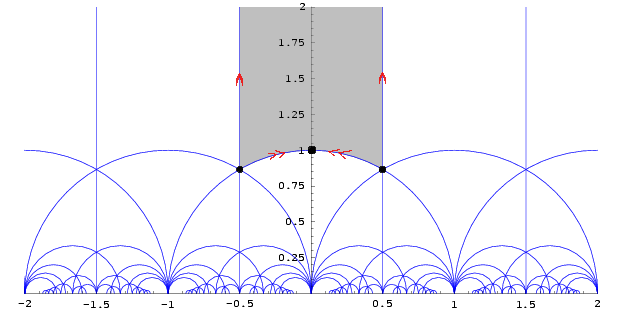
\includegraphics[width=9cm]{Immagini/ModularGroup-FundamentalDomain-01.png}
    \caption{Dominio fondamentale e qualche geodetica.}
    \label{SemipianoPoincare}
\end{figure}

\noindent
Le geodetiche sono le intersezioni dell'oggetto con rette verticali o semicirconferenze perpendicolari all'asse $x$.
Chiamiamo $\Mc$ questo spazio.
\end{definition}
\begin{example}[Geodetiche sul piano di Poincar\'e]
A parte le geodetiche corrispondenti a rette verticali, ogni geodetica che incontra la regione lo fa passando per l'asse $y$ (e quindi lo fa ad un certo angolo). Possiamo associare ad ogni coppia punto di $\Mc$ e angolo una geodetica di $\Mc$ (quella passante per il punto che incontra la verticale a quell'angolo)
\[\Mc\times S^1\ni ((x,y),\theta)\mapsto g_t((x,y),\theta).\]
Sia $\Sigma=\cpa{x=0,y>1}\times S^1$. \`E possibile definire $P_\Sigma$ e si da il caso che questa mappa di Poincar\'e \`e pi\`u facile da studiare rispetto al sistema originale.
\end{example}

